\documentclass[adobefonts, nocap]{ctexart}
\usepackage{amsmath}
\usepackage{amsfonts}
\usepackage{listings}
\usepackage{xcolor}
\usepackage{graphicx}
\usepackage{siunitx}
\usepackage{hyperref}
\hypersetup{
  colorlinks = true,
  linkcolor = blue,
  unicode = true
}
\lstset{
  language = C,
  basicstyle = \small\ttfamily,
  keywordstyle = \small\ttfamily\color{red},
  stringstyle = \color{gray},
  numbers = left,
  numberstyle = \small,
  numbersep = 5pt,
  frame = leftline,
  showstringspaces = false
}
\def\D{\mathrm{d}}
\begin{document}
  \title{计算机系统结构第三次作业}
  \author{李雨田\hspace{1em}2010012193\hspace{1em}计14}
  \maketitle
  \section*{3.8}
    如图所示,可以先计算$A_{i}\times B_{i}$, $i\in \{1,2,3\}$,在计算$A_{4}\times B_{4}$之前先计算出$A_{1}\times B_{1}+A_{2}\times B_{2}$,然后再算出剩下的值.

    \begin{center}
      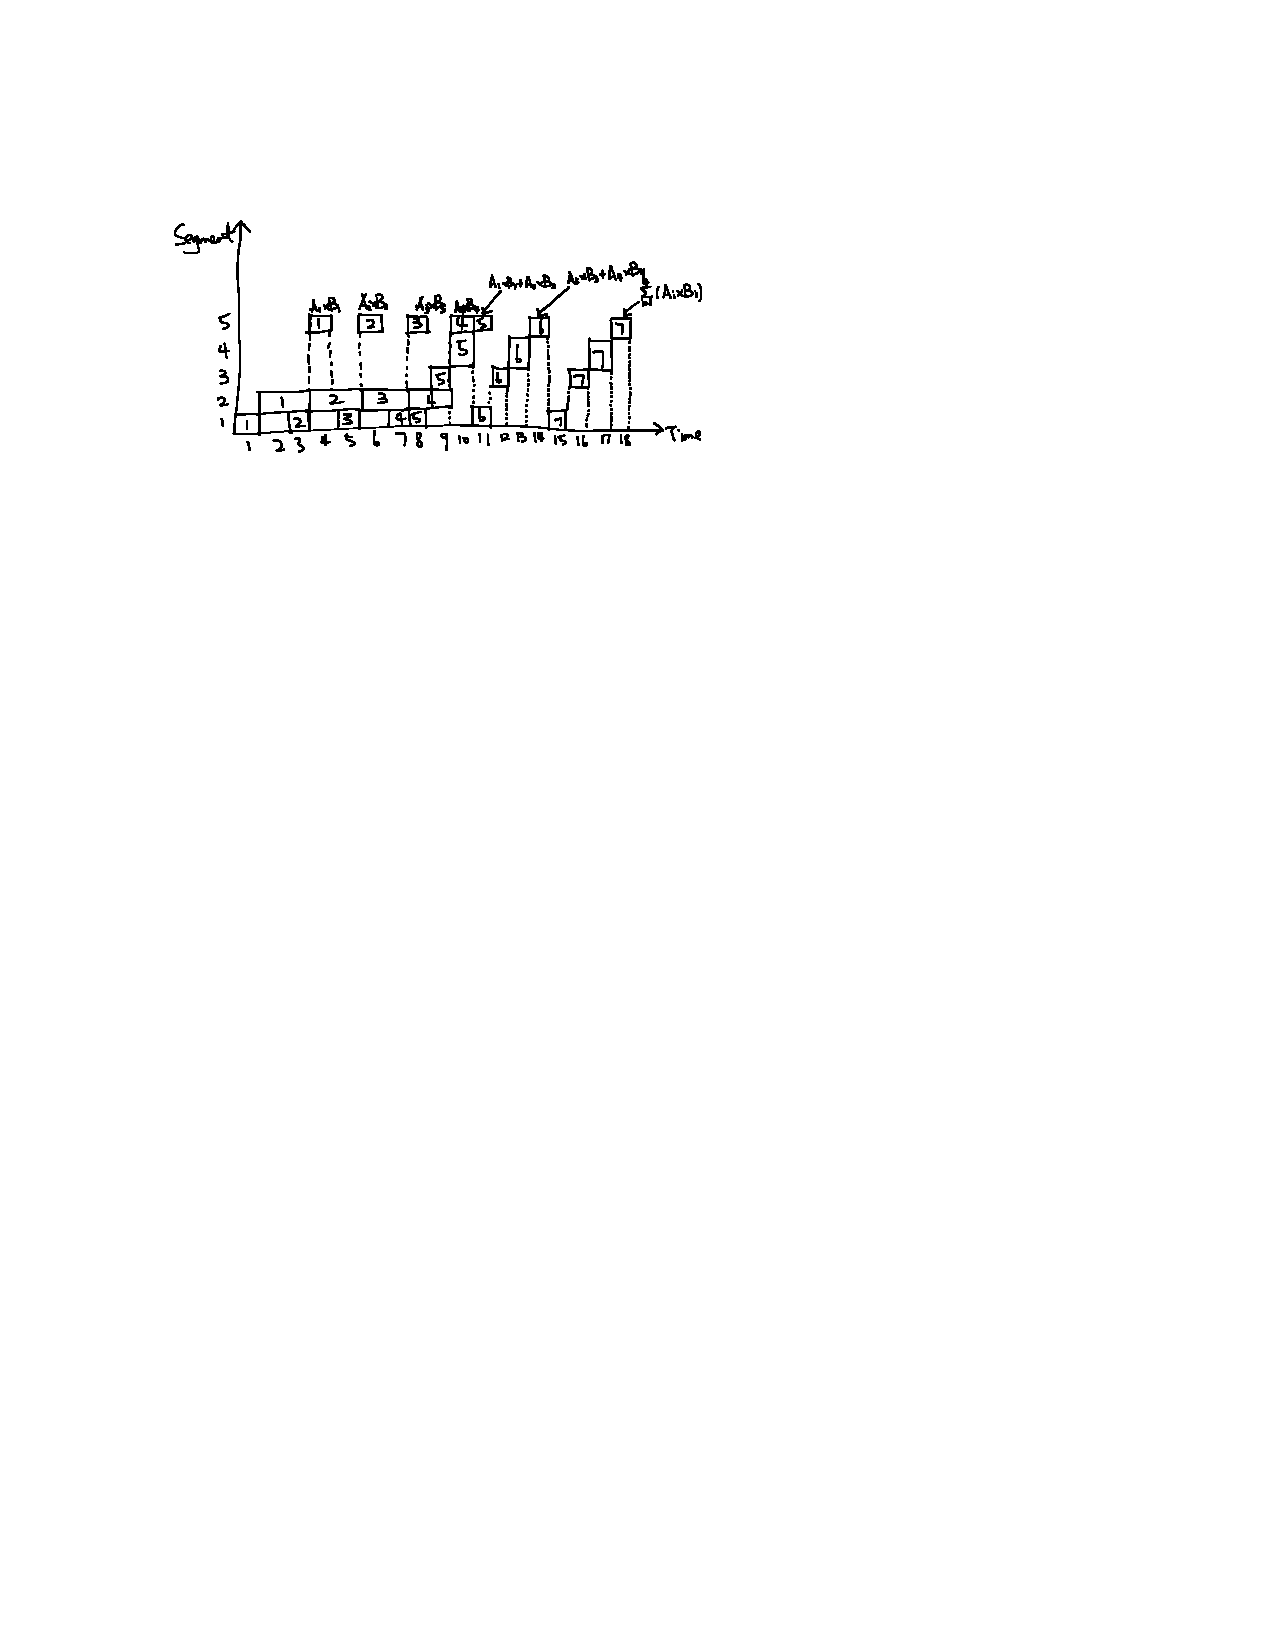
\includegraphics[width=10cm]{1-crop.pdf}
    \end{center}

    在$18$个$\Delta t$时间中,给出了$7$个结果,所以吞吐率为
    \[
      TP=\frac{7}{18\Delta t}.
    \]

    如果不适用流水线,产生$7$个结果总共需要时间$(4\times 4+3\times 4)\Delta t=28\Delta t$,所以加速比为
    \[
      S=\frac{28\Delta t}{18\Delta t}=\frac{14}{9}.
    \]

    流水线的效率可由阴影区的面积和总面积的比值求得
    \[
      E=\frac{28}{5\times 18}=\frac{14}{45}.
    \]
  \section*{3.9}
    根据预约表,可以得到禁止表
    \[
      F=\{1,3,4,8\}.
    \]

    写出初始冲突向量
    \[
      C_{0}=(10001101).
    \]

    再根据初始冲突向量可以画出状态转换图.

    \begin{center}
      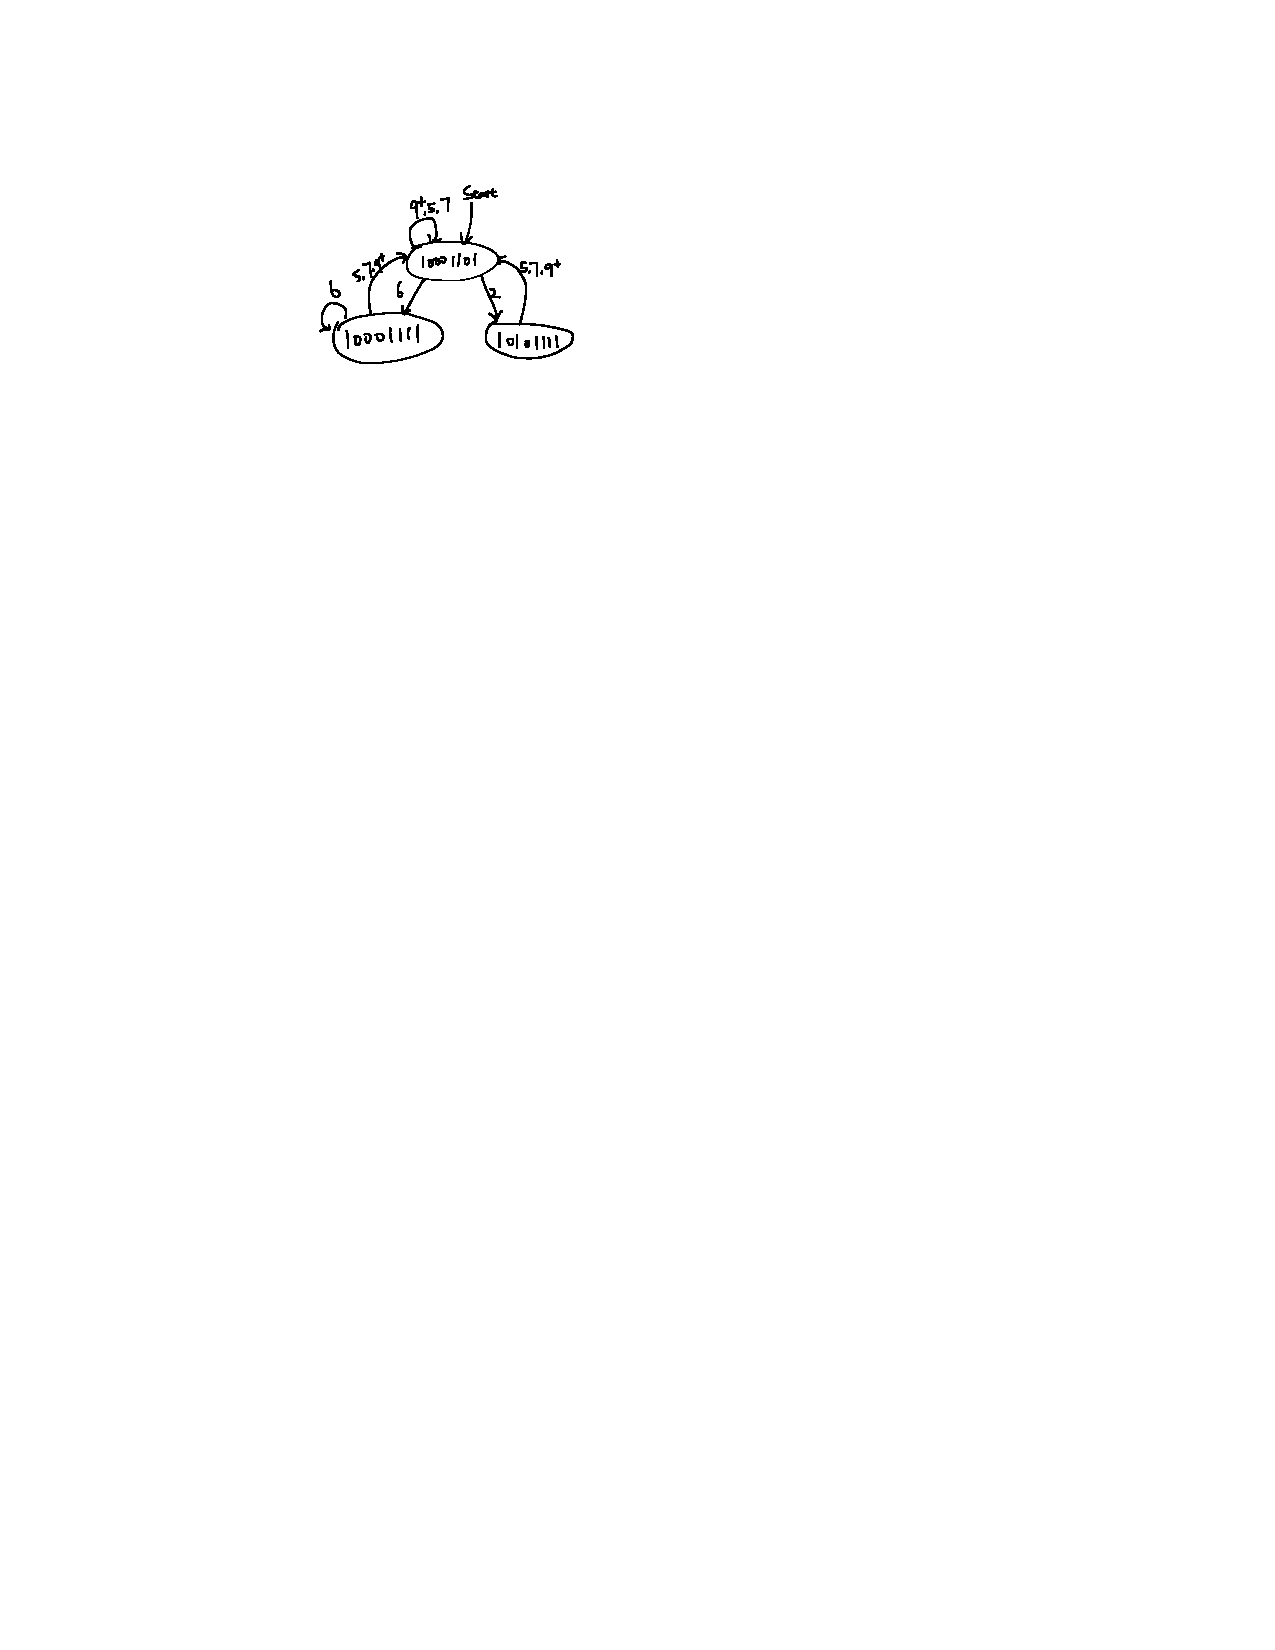
\includegraphics[width=10cm]{2-crop.pdf}
    \end{center}

    可以看出$(2,5)$是最优的调度策略,平均时间间隔是$3.5\Delta t$,即可得吞吐率
    \[
      TP=\frac{1}{3.5\Delta t}=\frac{2}{7\Delta t}.
    \]

    如果连续输出$6$个任务,分别相隔$2\Delta t, 5\Delta t, 2\Delta t, 5\Delta t, 2\Delta t, 5\Delta t$进入流水线,最后一个任务执行还需要时间$9\Delta t$,总共时间为$30\Delta t$.实际吞吐率为
    \[
      TP=\frac{6}{30\Delta t}=\frac{1}{5\Delta t}.
    \]

    实际吞吐率总是小于理论上的最大吞吐率,这个结论得到验证.
  \section*{3.10}
    使用相同的流程,首先根据预约表得到禁止表
    \[
      F=\{1,3,6\}.
    \]

    写出初始冲突向量
    \[
      C_{0}=(100101).
    \]

    再根据初始冲突向量可以画出状态转换图.

    \begin{center}
      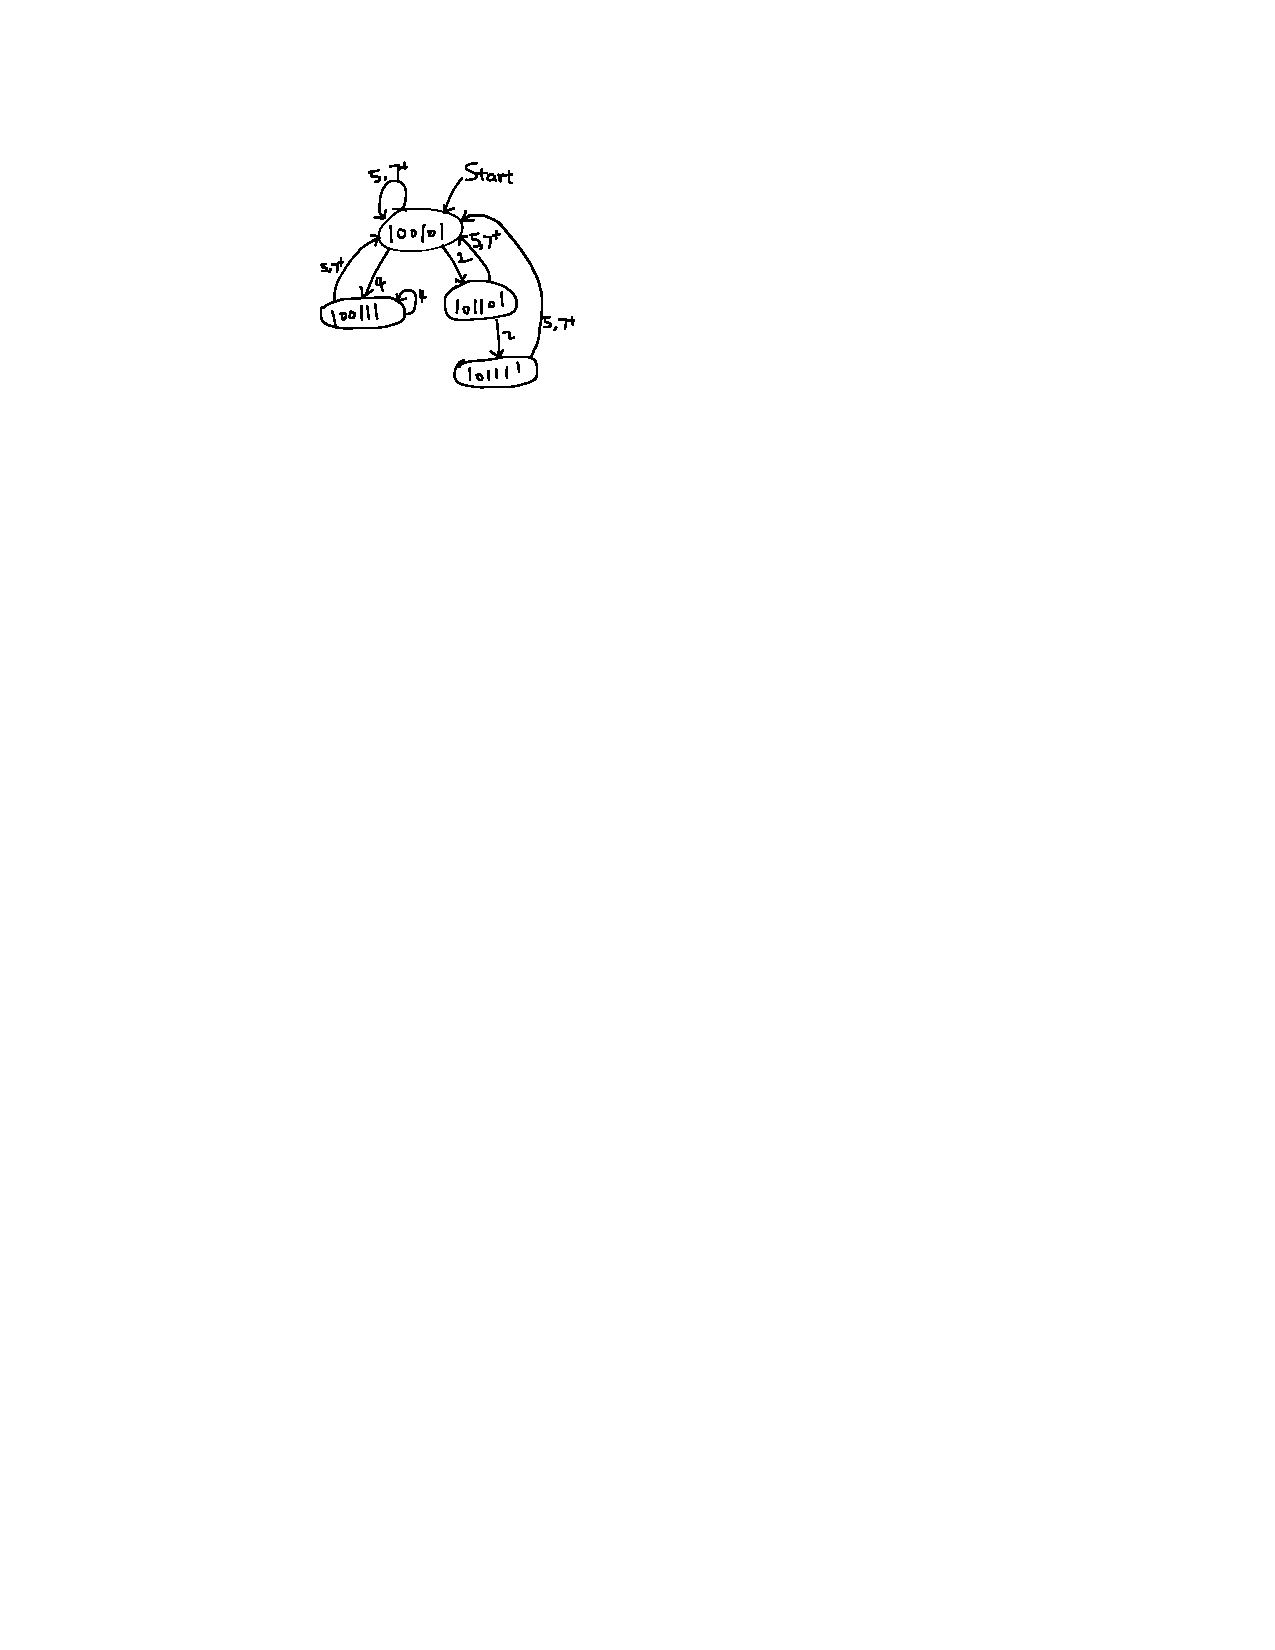
\includegraphics[width=10cm]{3-crop.pdf}
    \end{center}

    可以看出允许不等时间间隔调度时,$(2,2,5)$是最优的调度策略,平均时间间隔是$3\Delta t$,可得到吞吐率
    \[
      TF=\frac{1}{3\Delta t}.
    \]

    等时间间隔调度时,最优调度策略是$(5)$,吞吐率
    \[
      TF=\frac{1}{5\Delta t}.
    \]

    连续输入$10$个任务时,采用不等时间间隔调度耗时$(2+2+5+2+2+5+2+2+5+2+7)\Delta t=36\Delta t$,实际吞吐率
    \[
      TF=\frac{10}{36\Delta t}=\frac{5}{18\Delta t},
    \]
    加速比为
    \[
      S=\frac{10\times 7\Delta t}{36\Delta t}=\frac{35}{18}.
    \]

    采用等时间间隔调度则耗时$(10\times 5+7)\Delta t=57\Delta t$,实际吞吐率
    \[
      TF=\frac{10}{57\Delta t},
    \]
    加速比为
    \[
      S=\frac{10\times 7\Delta t}{57\Delta t}=\frac{70}{57}.
    \]
  \section*{3.11}
    如果不使用任何其他定向硬件,可以画出流水线时空图如下.进行一次循环需要$18$个时钟周期,并且两次循环只有$1$个时钟周期的重叠.根据程序源代码不难算出总共需要循环$99$
    次,所以整体执行需要$98\times (18-1)+18=1684$个时钟周期.

    这里用I表示IF, D表示ID, E表示EX, M表示MEM, W表示WB.

    {\footnotesize
      \center{
        \begin{tabular}{l||c|c|c|c|c|c|c|c|c|c|c|c|c|c|c|c|c|c}
          LW        & I & D & E & M & W & ~ & ~ & ~ & ~ & ~ & ~ & ~ & ~ & ~ & ~ & ~ & ~ & ~ \\
          DADDIU R1 & ~ & I & I & I & D & E & M & W & ~ & ~ & ~ & ~ & ~ & ~ & ~ & ~ & ~ & ~ \\
          SW        & ~ & ~ & ~ & ~ & I & I & I & D & E & M & W & ~ & ~ & ~ & ~ & ~ & ~ & ~ \\
          DADDIU R2 & ~ & ~ & ~ & ~ & ~ & ~ & ~ & I & D & E & M & W & ~ & ~ & ~ & ~ & ~ & ~ \\
          DSUB      & ~ & ~ & ~ & ~ & ~ & ~ & ~ & ~ & I & I & I & D & E & M & W & ~ & ~ & ~ \\
          BNEZ      & ~ & ~ & ~ & ~ & ~ & ~ & ~ & ~ & ~ & ~ & ~ & I & I & I & D & E & M & W \\
          LW2       & ~ & ~ & ~ & ~ & ~ & ~ & ~ & ~ & ~ & ~ & ~ & ~ & ~ & ~ & I & I & I & I \\
        \end{tabular}
      }
    }

    如果有正常的定向路径,可以画出流水线时空图如下.这里采用的是预测分支失败的策略,但是每次循环都是分支成功,所以在执行BNEZ后的指令时,
    第一次IF得到的指令会失败,需要重新IF得到正确的指令.这里进行一次循环需要$11$个时钟周期,两次循环有$3$个周期的重叠.整体需要$98\times (11-3)+11=795$个时钟周期.

    {\footnotesize
      \center{
        \begin{tabular}{l||c|c|c|c|c|c|c|c|c|c|c}
          LW        & I & D & E & M & W & ~ & ~ & ~ & ~ & ~ & ~ \\
          DADDIU R1 & ~ & I & D & D & E & M & W & ~ & ~ & ~ & ~ \\
          SW        & ~ & ~ & ~ & I & D & E & M & W & ~ & ~ & ~ \\
          DADDIU R2 & ~ & ~ & ~ & ~ & I & D & E & M & W & ~ & ~ \\
          DSUB      & ~ & ~ & ~ & ~ & ~ & I & D & E & M & W & ~ \\
          BNEZ      & ~ & ~ & ~ & ~ & ~ & ~ & I & D & E & M & W \\
          ???       & ~ & ~ & ~ & ~ & ~ & ~ & ~ & I & I & D & E \\
        \end{tabular}
      }
    }

    如果有一个单周期延迟分支.注意到现在仅有的延迟来自LW,所以可以把LW指令放在BNEZ之前进行执行,把DADDIU R1放在BNEZ之后的延迟槽进行执行.由于循环的时候分支总是
    成功,这样就把LW和DADDIU R1之间的一个时钟周期的延迟利用了起来,延迟槽指令的结果也能每次都被采用.流水时空图如下.

    这样的话,一次循环只要$10$个时钟周期,两次循环有$4$个周期的重叠,中间循环的$98$次共需要$98\times (10-4)=588$个时钟周期.但是第一次循环的LW和DADDIU R1之间的延迟是
    无法避免的,多需要$3$个时钟周期,最后一次循环要等流水线里的操作完全执行完,还需要$9$个周期.最后一次循环虽然BNEZ前仍然有LW,但是BNEZ会分支失败,所以此LW指令在最后一步
    WB时要取消,不能写回寄存器.这个LW也是跟其他方式相比,多执行的唯一一条指令.这里总共需要$600$个时钟周期.

    {\footnotesize
      \center{
        \begin{tabular}{l||c|c|c|c|c|c|c|c|c|c}
          SW        & I & D & E & M & W & ~ & ~ & ~ & ~ & ~ \\
          DADDIU R2 & ~ & I & D & E & M & W & ~ & ~ & ~ & ~ \\
          DSUB      & ~ & ~ & I & D & E & M & W & ~ & ~ & ~ \\
          LW        & ~ & ~ & ~ & I & D & E & M & W & ~ & ~ \\
          BNEZ      & ~ & ~ & ~ & ~ & I & D & E & M & W & ~ \\
          DADDIU R1 & ~ & ~ & ~ & ~ & ~ & I & D & E & M & W \\
          ???       & ~ & ~ & ~ & ~ & ~ & ~ & I & D & E & M \\
        \end{tabular}
      }
    }
  \section*{Q1}
    如果MEM阶段是load到寄存器B,且ID阶段要读寄存器B,那么需要定向.
  \section*{Q2}
    如果MEM阶段是load到寄存器r,且ID阶段是ALU指令读寄存器r,那么需在EX阶段插入气泡,并且ID阶段指令保留一个周期.
  \section*{Q3}
    只需要从内存中读取一个数存放到寄存器中,并且立马读取它,那么就会需要从MEM阶段定向过来.
    很容易写出如下代码. \\
    LW R1, 0(R2) \\
    DADDIU, R1, R1, \#1

\end{document}
